\section{Previous Work}
The following section will outline some of the previous work which has been considered in order to come up with our solution.

\subsection{Compositional Pattern Producing Networks}
\label{sec:cppn}
Compositional Pattern Producing Networks(CPPN) are a type of Artificial Neural Networks(ANN) introduced by Kenneth Stanley\cite{Stanley2007}.
CPPNs use function composition in an effort to obtain repetition, symmetry, and regularities in the produced phenomes.
An example of how composing functions can obtain multiple regularities can be seen on figure~\ref{fig:cppn}.
\begin{figure}[ht]
\centering
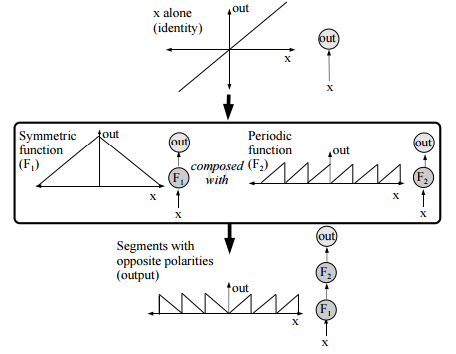
\includegraphics[width=.9\columnwidth]{cppn}
\caption{Composing two functions to obtain a single function which has multiple regularities \cite{Stanley2007}}
\label{fig:cppn}
\end{figure}

CPPNs are of interest to our solution because of their symmetry producing properties.
%Stanley presented some experiments which used CPPNs to evolve two-dimensional images.
%The input to these networks were the x- and y-coordinates of the images, and the single output produced by the CPPN was used to colour the pixel at the given coordinate.

\subsection{Computer evolved tables}
\todo[inline]{Change this title?}
Evolutionary Algorithms have been used to develop similar solutions before. Examples of previous  applications are tables[See~figure~\ref{fig:hornby_tables}] where the optimisation parameters were height of the support structure, stability of the structure, and maximization of surface area.
\begin{figure}[ht]
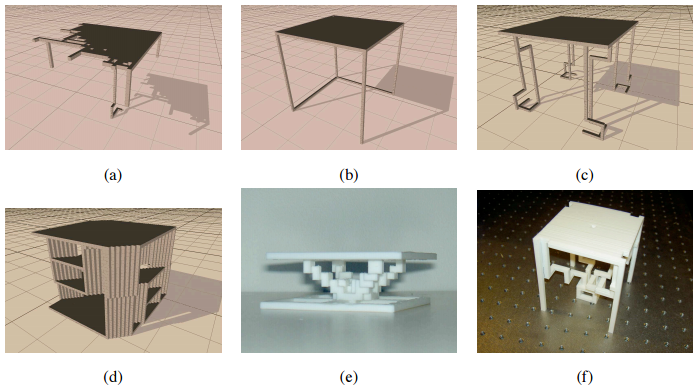
\includegraphics[scale=.6]{content/img/tables}
\caption{Image of Hornby tables\cite{paper:ev4}}
\label{fig:hornby_tables}
\end{figure}

While the evolution of tables has some similarities to seating they are inherently
different in the sense that maximized surface area might not be ideal for a
chair.
Neither would very high legs be optimal, since the physical attributes of humans
usually constrain us to some specific height range which is optimal for the
average persons seating comfort.

\subsection{Interactive Evolutionary Computation}
Takagi describes in his survey from 2001\cite{Takagi2001} how there are some \emph{``systems whose optimization indexes are difficult to specify''}\cite[p.~1275]{Takagi2001}.
For such systems, which include systems whose evaluation is aesthetic in nature, it is beneficial to use a human subject to evaluate the outcome of the Evolutionary Computation(EC).
This method is called Interactive Evolutionary Computation(IEC).

Some sort of IEC if of interest to our solution, since we would like to guide the evolution. 

\subsection{Evolving 3D objects with CPPNs}
In their paper from 2011 Klune and Lipson describe how they use CPPNs to evolve 3-dimensional objects\cite{Clune:2011:EOG:2078245.2078246}.
They describe how they encode the 3D objects with CPPNs by feeding the CPPN with three inputs, one each for the x-, y-, and z-coordinates of a 3D voxel space.
The single output of the CPPN for the given coordinates is checked against a threshold, and if it is above the threshold then the voxel in those coordinates is considered full, otherwise it is considered empty\cite[p.~5]{Clune:2011:EOG:2078245.2078246}.
They combine this encoding with IEC to evolve symmetrical 3D images, see figure~\ref{fig:3dobjects}.
\begin{figure}[ht]
\centering
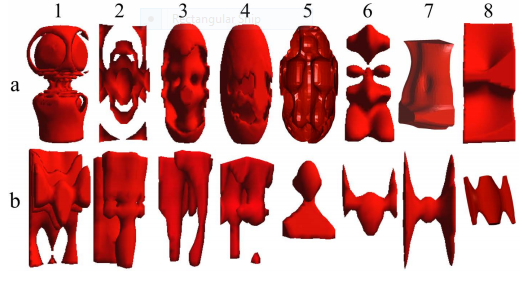
\includegraphics[width=.9\columnwidth]{3d_cppn}
\caption{Examples of the 3D images presented in \cite{Clune:2011:EOG:2078245.2078246}}
\label{fig:3dobjects}
\end{figure}

